%\pdfoutput=1

\documentclass{l4proj}

%
% put any packages here
%
\usepackage{float}
\usepackage[labelfont=bf]{caption}

\usepackage{subfigure}

\usepackage{cleveref}

\setcounter{tocdepth}{3}
\usepackage{graphicx}
\usepackage{algorithmic}
\usepackage[ruled,vlined]{algorithm2e}
\usepackage{url}
\usepackage{alltt}
\urldef{\mailsa}\path|pat@dcs.gla.ac.uk|
\newcommand{\keywords}[1]{\par\addvspace\baselineskip
\noindent\keywordname\enspace\ignorespaces#1}
\newlength{\halftextwidth}
\setlength{\halftextwidth}{0.47\textwidth}

\usepackage{amsopn}
\DeclareMathOperator{\mod}{mod}

\newtheorem{theorem}{Theorem}
\newtheorem{definition}{Definition}


\renewcommand{\figurename}{Fig.}
\Crefformat{figure}{#2Fig.~#1#3}
\Crefmultiformat{figure}{Figs.~#2#1#3}{ and~#2#1#3}{, #2#1#3}{ and~#2#1#3}

\usepackage{listings}
\usepackage{color}

\definecolor{dkgreen}{rgb}{0,0.6,0}
\definecolor{gray}{rgb}{0.5,0.5,0.5}
\definecolor{mauve}{rgb}{0.58,0,0.82}

\lstset{
  %frame=tb,
  language=Java,
  %aboveskip=3mm,
  %belowskip=3mm,
  showstringspaces=false,
  columns=flexible,
  %basicstyle={\small\ttfamily},
  basicstyle=\scriptsize,     % the size of the fonts that are used for the code  
  numbers=left,
  stepnumber=1,
  numberstyle=\small\color{gray},    % the size of the fonts that are used for the line-numbers
  numbersep=10pt,             % how far the line-numbers are from the code
  keywordstyle=\color{blue},
  commentstyle=\color{dkgreen},
  stringstyle=\color{mauve},
  breaklines=true,            % sets automatic line breaking
  breakatwhitespace=false,    % sets if automatic breaks should only happen at whitespace
  showstringspaces=false,     % Don't show underscores as space characters
  %tabsize=4,
  frame=trBL,                 % adds a frame around the code
  frameround=fttt,
  captionpos=b,               % sets the caption-position to bottom
}

\begin{document}

\title{Animating a Sudoku solver}
\author{Gabriel I. Stratan}
\date{November 18, 2015}
\maketitle

\begin{abstract}
Sudoku is a popular puzzle played all over the world. It consists of filling in a 9x9 grid such that every row, column and 3x3 sub-grids have different digits from 1 to 9. Solving the puzzle will make use of the all-different algorithm from Constraint Programming for which an implementation will be provided. Finally, the program will animate all the steps done by the algorithm.
\end{abstract}

\educationalconsent
%
%NOTE: if you include the educationalconsent (above) and your project is graded an A then
%      it may be entered in the CS Hall of Fame
%
%\tableofcontents
%==============================================================================
\chapter{Introduction}
\label{intro}
\pagenumbering{arabic}

\section{Aims}
Teaching constraint programming, need for visualisations

\section{Background}

\section{Sudoku}
\noindent Sudoku is a puzzle 

\section{Constraint Programming}
\noindent Every Constraint Satisfaction Problem (CSP) has variables with domains and constraints associated to them. To start solving Sudoku puzzles, we have to come up with a model representation of the problem. For the purpose of this exercise, there will be 81 variables representing the 9x9 cells in the Sudoku grid, each with an initial domain of integers from 1 to 9. As all the initial puzzles start with a partially completed grid, values that are known will be reflected as variables with an initial domain of one digit, the known value. Such variables will therefore keep their initial domain throughout the algorithm, as no other values are present in their domain.

\noindent The constraints for a Sudoku puzzle can be expressed in natural language as such: “digits may not appear twice in the same row, column or 3x3 subregions”. The rules of the puzzle highlight the need of thinking in terms of 9 rows, 9 columns and 9 subregions, each of them having digits from 1 to 9 with no repetition. We can create 36 not equals constraints between the 9 variables of each row, column, subregions times 27 such regions for a total of 972 constraints between two variables. This would be highly inefficient, hence the need for a better approach. A better approach is to use 27 all-different constraints, one for each row, column and subregions. Each constraint contains 9 variables that should take different values. As each variable is part of a row, column and subregion at the same time, it will therefore be involved in 3 constraints.

\noindent Initial puzzles are always partially completed with enough values that by the end of the game there will be a single unique solution to the puzzle. 

\noindent We get to the solution by running the alldifferent algorithm on rows, columns and subregions to remove values from the domain of the variables. Initially, the known values given at the start of the puzzle will be removed from the domains of possible values in the variables that are part of the same row, column or subregion. As the algorithm progresses, we will eventually remove enough values from the domain of a variable until we are left with a single value that represents the correct answer for that position. Once a value is found, there is a waterfall-like effect across the puzzle as we propagate the knowledge across the grid. The propagation takes place across all the variables that are in the same row, column and subregion with the one just solved. This will keep the 3 constraints in a consistent state, as all the variables will have valid remaining domains not containing any already solved values.

\noindent The algorithm is intelligent in a sense that it mimics the thinking of humans when solving a Sudoku puzzle. At some stages of the game we have enough information to know that two particular values will fill two cells, but no information about which value corresponds to which cell. This problem is what makes some Sudoku puzzles so hard to solve.

\noindent Humans and the alldifferent algorithm are smart enough to use this information to their advantage and remove the two values from the domains of the adjacent variables. By using this technique, we can ensure the progress of the algorithm towards a solution, even though we still don’t know which two variables take which two values. It is good to note that although humans may choose a guessing approach to continue towards a solution, the alldifferent algorithm performs no guessing and works only with the information about the current state of the puzzle.

\section{The Alldifferent Constraint}
Review Regin’s paper and explain how constraint works

Example of  its usage and how it works (maybe 5 variables with domains)

 
\chapter{Algorithms for AllDiff}
\section{Ford Fulkerson}
Having a maximum matching for our graph, the next step in the alldifferent algorithm is to turn the previously undirected graph, into a directed one. The matches resulted from the Ford Fulkerson algorithm are assigned a direction from the 1 to 9 values to the corresponding cells of the Sudoku row. The edges that remain unused in the matching are given a direction from left to right (i.e. from the Sudoku cells of the row to the 1-9 values).

\noindent // write that we delete S/T nodes and corresponding edges

\noindent Ford Fulkerson's algorithm for finding a maximum flow in a graph is shown in algorithm \ref{FordFulkersonPC}. The $Ford Fulkerson$ procedure on line 1 takes a graph $G$ as an argument and represents the start of the algorithm. The graph passed as an argument holds information about the capacity of each edge. Line 3 stores the capacity of the graph $G$ in a global two-dimensional integer array. The capacity of an edge between vertices $u$, $v$ can be found out in $capacity[u][v]$. Line 4 declares an integer $n$ used to store the number of vertices in the given graph. Lines 5 and 6 declare two integers called $source$ and $sink$ representing the first and the last vertices in the given graph.

\noindent In line 7 we declare a vertex-indexed array $pred$ that is used to store references to the previous vertex discovered in the breadth-first search tree. Line 8 declares a vertex-indexed array $visited$ used to keep track if a vertex has already been visited in the breadth-first search procedure. Line 9 declares a queue of integers $Q$ used to store \textbf{XXX}.

\noindent The algorithm consists of repeated calls to the breadth-first search procedure (line 10). In line 11, as long as the breadth-first search procedure finds \textbf{shorter augmenting paths?} we call the update procedure to update the capacities of the edges.

\noindent The $breadth-first search$ procedure starts at line 12 and takes a graph $G$ as an argument. In lines 14 to 16, the queue $Q$, $pred$ and $visited$ array are reset to have default values.

\noindent The breadth-first search calls always start from the first vertex, representing the source. This vertex is enqueued on queue $Q$ in line 17 and is marked as visited in line 18.

\noindent Lines 19 to 26 contain a loop performing changes on the queue $Q$ that is used to store an augmenting path. The loop starts on line 20 by dequeuing a vertex from the queue $Q$ and storing it in $v$. Line 21 forces the breadth-first search procedure to return $true$ when we reach the last vertex in the graph, the sink. Lines 22 to 26 contain a loop over \textbf{all the vertices} $w$ in the graph. In line 23 we check to see if the discovered vertex $w$ hasn't been already visited and we consider it if it still has available capacity. Line 24 stores the parent value of $w$ in the augmenting path. Line 25 enqueues the discovered vertex $w$ on the queue $Q$ and marks it as visited in line 26. Finally, the breadth-first search procedure returns $false$ in case \textbf{of no augmenting path found?}.

\noindent The $update$ procedure at line 28 is used to update the capacities in the graph to reflect the found paths. Line 30 declares an integer $f$ used to store the \textbf{difference/delta}. Line 31 declares an integer $v$, initially representing the last vertex in the graph called the sink. Lines 32 to 35 contain a loop that updates the capacities of the edges \textbf{in the augmenting path?}. Line 33 uses the integer $u$ to store a vertex that is the neighbour of vertex $v$ \textbf{in the path}, so that together they make an edge. Lines 34 and 35 updates the flow along the edge from $u$ to $v$ and $v$ to $u$ by the found difference.

\noindent The $minCost$ procedure at line 36 is used to find the minimum cost, in terms of capacity used, from the sink \textbf{to the source?}. Line 38 declares an integer $minCost$ used to represent the current value of the minimum cost, and it has a very large number at the time of its initialization. Line 39 declares an integer variable $v$ used to store vertices. The variable $v$ is initialized as the last vertex in the graph called the sink. Lines 40 to 42 contains a \textbf{loop over the parent vertices} of $v$. Line 41 updates the value of the minCost variable \textbf{to the minimum}. The $minimum$ procedure returns the minimum of two given integers. Line 42 updates the value of integer $v$ to \textbf{its parent}. At the end of the $minCost$ procedure, we return the value of the currently found $minCost$ variable.

\begin{algorithm}
\DontPrintSemicolon
\nl $\textbf{void} ~FordFulkerson(\textbf{Graph}~G)$ \;
\nl \Begin{
\nl $\textbf{Global} ~ \textbf{int} ~ capacity[][] \gets getCapacity(G)$ \;
\nl $\textbf{Global} ~ \textbf{int} ~ n \gets |V(G)|$ \;
\nl $\textbf{Global} ~ \textbf{int} ~ source \gets 0$ \;
\nl $\textbf{Global} ~ \textbf{int} ~ sink \gets n-1$ \;
\nl $\textbf{Global} ~ pred \gets ~new~\textbf{int}[n]$ \;
\nl $\textbf{Global} ~ visited \gets ~new~\textbf{boolean}[n]$ \;
\nl $\textbf{Global} ~ Q \gets ~new~\textbf{Queue}()$ \;
\nl \While {$bfs(G)$}{
\nl $update()$ \;
}

} %begin FordFulkerson

\;
\nl $\textbf{boolean} ~bfs(\textbf{Graph} ~ G)$ \;
\nl \Begin{
\nl $clear(Q) $ \;
\nl $fill(pred, -1) $ \;
\nl $fill(visited, false) $ \;
\nl $enqueue(source, Q) $ \;
\nl $visited[source] \gets ~true $\;
\nl \While {$(\neg isEmpty(Q))$}{
\nl $\textbf{int} ~ v \gets dequeue(Q) $ \;
\nl \lIf {$v = ~ sink $}{ $\textbf{return} ~ true $ }

\nl \For {$w \gets ~ 0 ~ to ~ n $}{
\nl \If {$\neg visited[w] ~ \textbf{and} ~ capacity[v][w] > 0$}{ 
\nl $ pred[w] \gets v$ \;
\nl $ enqueue(w, Q)$ \;
\nl $ visited[w] \gets true$ \;
} %if
} %for
} %while
\nl $\textbf{return} ~ false $ \;
} %begin bfs

\;

\nl $\textbf{void} ~update()$ \;
\nl \Begin{

\nl $\textbf{int} ~ f \gets minCost()$ \;
\nl $\textbf{int} ~ v \gets sink $ \;

\nl \While {$pred[v] \neq -1$}{
\nl $\textbf{int} ~ u \gets pred[v] $ \;
\nl $capacity[u][v] \gets capacity[u][v] - f $ \;
\nl $capacity[v][u] \gets capacity[v][u] + f $ \;
} %while

} %begin updateR

\;

\nl $\textbf{int} ~minCost()$ \;
\nl \Begin{

\nl $\textbf{int} ~ minCost \gets \infty $ \;
\nl $\textbf{int} ~ v \gets sink $ \;

\nl \While {$pred[v] \neq -1$}{
\nl $minCost \gets minimum(minCost, capacity[pred[v]][v])$ \;
\nl $v \gets pred[v]$ \;
}
\nl $\textbf{return} ~ minCost$ \;
} %begin updateR

\caption{Ford Fulkerson}
\label{FordFulkersonPC}
\end{algorithm}

\clearpage
\section{Tarjan algorithm}
Now that all the edges from the graph are directed, the next step in the alldifferent algorithm is to find the strongly connected components of the graph. In order to do this, we introduce now Tarjan’s algorithm for finding strongly connected components  (SCCs) in a given graph G.

\noindent The algorithm starts by visiting every node in the directed graph in a depth first search manner. During the search, nodes are added to a stack in the order they are discovered only if they were not already part of the stack. 

\noindent Backtracking is triggered when we reach a node that is upper compared to our previous node (if(min < low[u])).  We know this by keeping record of the upmost node reachable from node u, including node u itself during each branch of the depth first search. We use low to denote the minimum index representing the upmost node in the branch.

\noindent If the current node is less than the upper node is less than the current index, it means that we have 

\noindent If the upper node is equal to the node we are currently visiting, then the algorithm just found a strongly connected component that contains all nodes on the stack starting from the top of it, until encountering the current node. The nodes are popped out of the stack and a SCC id/index is assigned to it for later use. Once the current node is reached, we increment the count of the SCCs to start filling a new SCC.

\noindent // write that there are no self loops / self edges (u!=i)
\cite{tarjan1972depth}



\noindent Tarjan's algorithm for finding strongly connected components is shown in algorithm \ref{TarjanPC}. The $Tarjan$ proceduce in line 1 takes a Graph $G$ as an argument and represents the start of the algorithm. The global integer $pre$ declared in line 3 is used to store \textbf{XXX}. The integer $components$ in line 4 keeps track of how many components were identified in the given graph. The integer $n$ in line 5 represents the number of vertices in the given graph.

\noindent In line 6 we introduce a Stack data structure that will hold all the vertices that are part of the same strongly connected component. Line 7 contains a declaration for the $stacked$ vertex-indexed array of booleans used to keep track if a vertex is present or not on the stack $S$.

\noindent An integer vertex-indexed array $id$ is declared in line 8 to store the id of the strongly connected component of each vertex. Line 9 declares a vertex-indexed array $low$ used to store the topmost reachable vertex in the depth-first search tree through a back edge.

\noindent Lines 10 and 11 contain a for loop that calls a procedure for performing depth first search on every vertex in the given graph that is not currently stacked.

\noindent Line 12 declares a recursive procedure for performing a depth-first search starting from vertex $u$ in graph $G$.

\noindent The procedure starts by pushing the vertex $u$ on the stack $S$ (line 14) and updating the value in the $stacked$ array (line 15) to reflect the change. Line 16 sets the vertex's $v$ value for $low$ to $pre$ \textbf{XXX} in line 16 to 17. Line 18 declares an integer $min$ that has an initial value \textbf{XXX}.

\noindent Lines 19 to 21 loop through every vertex $v$ that is a neighbour of vertex $u$. The procedure $N(u, G)$ on line 19 returns a list of neighbouring vertices of a given vertex, not including the given vertex. If the discovered neighbour $v$ is not currently on the stack $S$, then we proceed to make a recursive call to the depth-first search function on the found vertex.

\noindent After the recursive call finishes processing the sub-tree of the neighbouring vertex $v$, $min$ gets updated on line 21 to store the topmost reachable vertex that could be the same, or even higher in the tree if a higher back-edge from $v$ was discovered.

\noindent Line 22 updates the topmost reachable vertex of vertex $u$ to reflect any changes after processing all the neighbouring vertices.

\noindent Line 23 declares an integer $v$ used to store a vertex that for the repeat-until loop in lines 24 to 28. The loop begins by popping vertices out of the stack $s$ on line 25. Each vertex $v$ found on the stack is assigned the current component id. Line 26 assigns the last leaf node of the graph as a topmost reachable vertex of vertex $v$ in order to mark it as already part of a component. The repeat-until loop in line 24 to 28 is runs until finding \textbf{XXX self edge?}.

\noindent The depth-first search procedure finishes on line 29 by updating the total number of strongly connected components discovered.

\clearpage

\begin{algorithm}
\DontPrintSemicolon
\nl $\textbf{void} ~Tarjan(\textbf{Graph}~G)$ \;
\nl \Begin{
\nl $\textbf{Global} ~ \textbf{int} ~ pre \gets 0 $ \;
\nl $\textbf{Global} ~ \textbf{int} ~ components \gets 0 $ \; %new
\nl $\textbf{Global} ~ \textbf{int} ~ n \gets |V(G)|$ \; %new
\nl $\textbf{Global} ~ S \gets ~new~\textbf{Stack}()$ \;
\nl $\textbf{Global} ~ stacked \gets ~new~\textbf{boolean}[n]$ \;
\nl $\textbf{Global} ~ id \gets ~new~\textbf{int}[n]$ \;
\nl $\textbf{Global} ~ low \gets ~new~\textbf{int}[n]$ \;

\nl \For {$u \in ~V(G)$}{
\nl \lIf {$\neg stacked[u]$}{ $ dfs(u, G) $ }
}
}
\;
\nl $\textbf{void} ~dfs(\textbf{int}~u, \textbf{Graph}~G)$ \;
\nl \Begin{
\nl $push(u, S) $ \;
\nl $stacked[u] \gets ~true $\;
\nl $low[u] \gets ~pre $ \;
\nl $pre \gets pre + 1$ \;
\nl $\textbf{int} ~ min \gets low[u] $ \;

\nl \For {$v \in ~ N(u, G)$}{
\nl \lIf {$\neg stacked[v]$}{ $dfs(v, G) $ }
\nl $ min \gets minimum(low[v], min) $
 }
\nl $ low[u] \gets minimum(low[u], min) $

\nl $\textbf{integer} ~ v $ \;

\nl \Repeat{\nl $v \neq u$}{
\nl $v \gets pop(S) $ \;
\nl $id[v] \gets components $ \;
\nl $low[v] \gets n $ \;
 }

\nl $ components \gets components + 1 $ \;

}
\caption{Tarjan's strongly connected components}
\label{TarjanPC}
\end{algorithm}

\chapter{AllDiff Demo}
implementation and usage

Explain how demo is used, what it shows, etc (NOT implementation)

 
\chapter{Implementation}
\noindent The Graphical User Interface (GUI) is inside a JLayeredPane which is a special swing component that allows components inside it to overlap according to their specified depth. In my implementation, the backmost layer contains a JPanel responsible for the drawn edges in the graph. The layer above contains the rest of the GUI represented by the Sudoku puzzle on the left hand side of the screen, and the vertices of the graph on the right hand side of the screen. By using a layered panel, the edges of the graph can be drawn behind the vertices.

\noindent The Sudoku Grid present on the left hand side of the screen is made up of 9 by 9 Sudoku Cells positioned at specific locations. When a new Sudoku Cell instance in made, its ith row and jth column number are passed as arguments to the constructor. Using the information related to its location in the grid, it is now possible to render the border of each cell. Initially all the top, left, bottom and right borders have a width of 1px. To represent the 3 by 3 sub-grids, specific borders are set to have a width of 2px. In the end, the 9 by 9 grid is given an overall thick border by specifying a width of 4px to the cells that are in the first and last columns and rows. All Sudoku Cells contain a JLabel with text retrieved from the Model denoting which possible values are still available for that particular cell.

\noindent Not visible to the human eye, a new Sudoku grid instance is drawn on top of the existing one, this time with all borders set to a width of 1px. The Sudoku Cells inside this second grid contain the same information about the state of the puzzle retrieved from the Model. Additional information such as a custom background will be applied to these cells as the algorithm progresses. Cells inside the second grid become visible once the user makes a selection. Once visible, the cells inside the selection are animated into their position inside the graph on the right hand side of the screen. When the user performs deselects his choice, the nice cells are animated back into their original position in the grid and become invisible again.
 
\noindent Particular attention was given to make the software thread safe. It is crucial that the application logic doesn’t make the Graphical User Interface unresponsive. To achieve this, the program will run on two threads, one main thread responsible with all the processing need to be done by the program, and the Event Dispatching Thread. 

\noindent The Event Dispatching Thread (EDT) is a background thread used to invoke Swing methods that change the GUI and listen to events associated to components. Most Swing components are not thread safe, therefore bugs such as race conditions could unexpectedly arise if it was to perform the actions from normal threads. The EDT acts as a queue of events that are performed sequentially.

\noindent Throughout the application, Timer objects are used to schedule repeated actions such as the fading out of the components or movement of the cells. The model contains a two-dimensional ArrayList of Timer objects that acts as a queue of animations. Timers on the same level start running at the same time until they all finish. Once all the timers on a level finish, the next level in the two-dimensional ArrayList is started, allowing us to queue a movement of a row after all the cells finish fading out.

\begin{figure}[H]
\centering
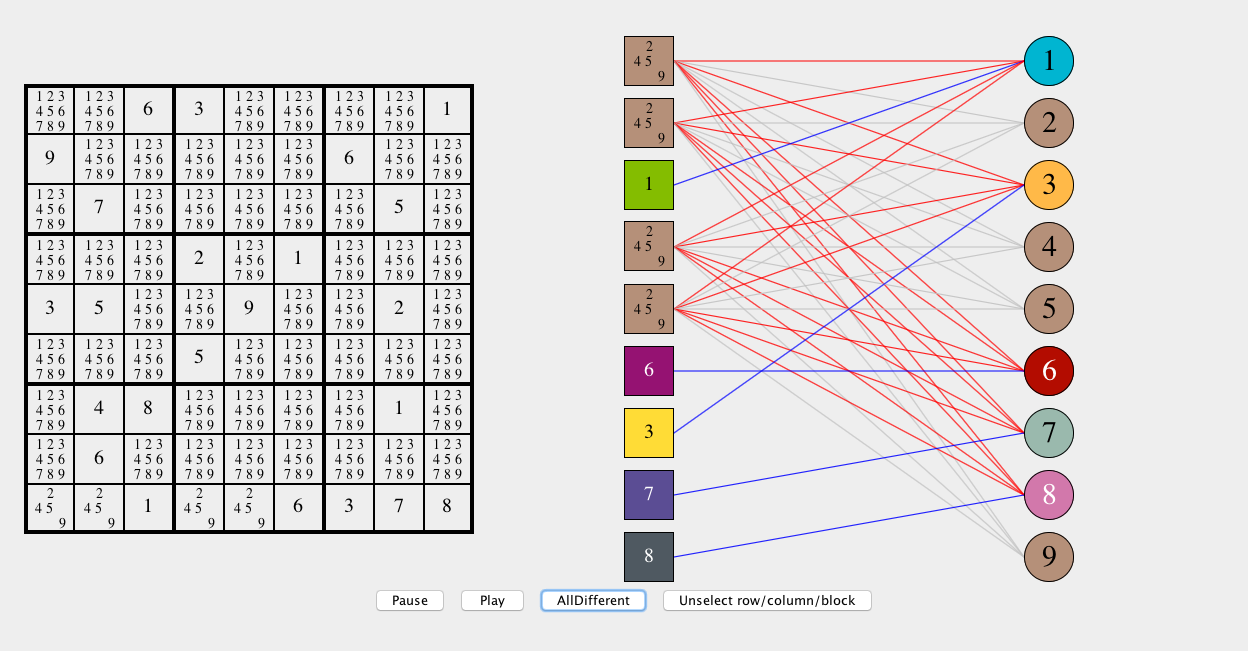
\includegraphics[width=13.2cm]{screenshot.png}
\caption{The state of the program after the all-different algorithm finishes on a row, in this case, the last one.}
\end{figure}

%\lstset{language=Java}

%\begin{figure}
%\lstset{caption={Implementation of Tarjan's algorithm %for finding strongly connected %components},label=codeTarjan}
%\lstinputlisting{Tarjan.java}
%\end{figure}

\chapter{Conclusion and Future Work}
\label{conclusion}
We have shown how to implement the all-different constraint.

%%%%%%%%%%%%%%%%
%              %
%  APPENDICES  %
%              %
%%%%%%%%%%%%%%%%
\begin{appendices}

\chapter{Running the Program}
An example of running from the command line is as follows:
\begin{verbatim}
      > javac *.java
      > java Sudoku
\end{verbatim}
This will open the application loaded with the hard Sudoku problem $/herald20061222H.txt$.

\noindent
\textbf{TODO}: what about the Choco3 library? add it to path? remove it?

\chapter{Proof of concept}

The following sequence of steps will provide a visual proof of the all-different algorithm. The following figures capture the user running the all-different algorithm on 5 predetermined rows, columns or 3x3 sub-grids. For demonstration purposes, the Sudoku instance used is $lockedset.txt$.

The sequence is as follows:
\begin{verbatim}
      > Open lockedset.txt Sudoku instance
      >
      > Select the 1st column
      > Run the all-different algorithm
      > Unselect
      >
      > Select the 5th row
      > Run the all-different algorithm
      > Unselect
      >
      > Select the 6th row
      > Run the all-different algorithm
      > Unselect
      >
      > Select the 4th 3x3 sub-grid
      > Run the all-different algorithm
      > Unselect
      >
      > Select the 1st column
      > Run the all-different algorithm
      > Unselect
\end{verbatim}

Alternatively, the user can press the $Show Demo$ button to run the same steps.

\begin{figure}[h]
\hfill
\subfigure[1st column after running the all-different algorithm]{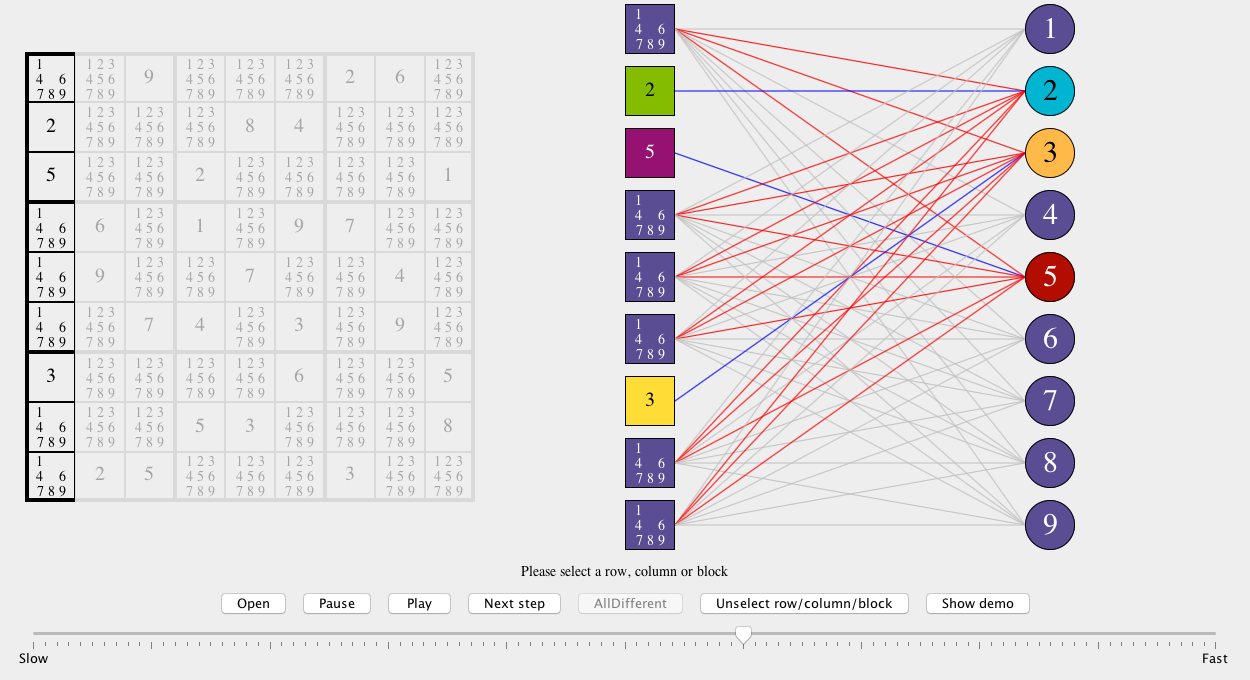
\includegraphics[width=8cm]{images/proof_of_concept/1.png}}
\hfill
\subfigure[5th row after running the all-different algorithm]{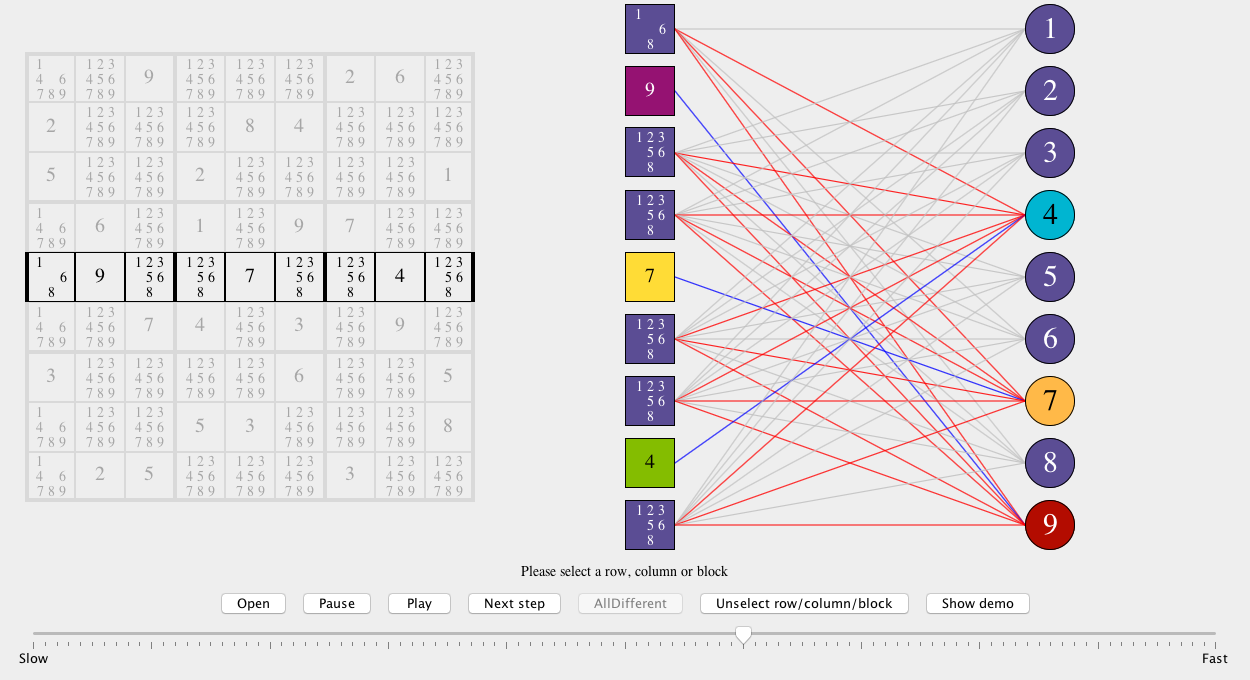
\includegraphics[width=8cm]{images/proof_of_concept/2.png}}
\vspace*{2cm}
\hfill
%\caption{Title for both}
%\end{figure}

%\begin{figure}[h]
\hfill
\subfigure[6th row after running the all-different algorithm]{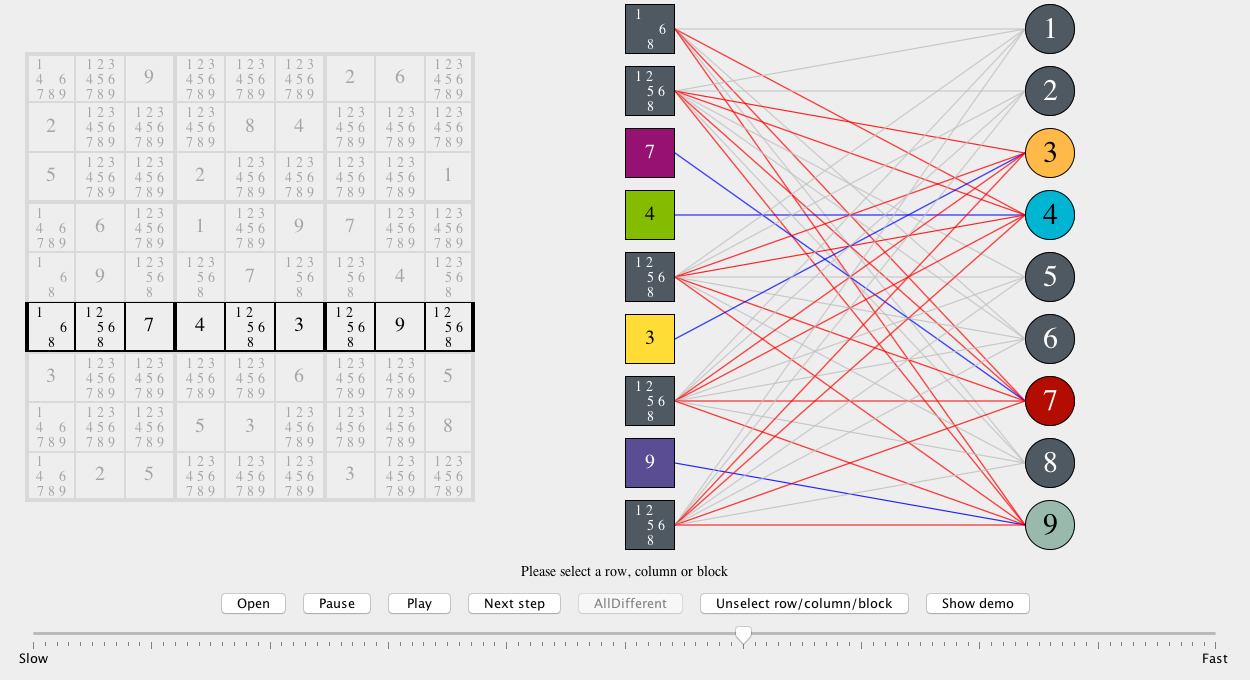
\includegraphics[width=8cm]{images/proof_of_concept/3.png}}
\hfill
\subfigure[4th 3x3 sub-grid after running the all-different algorithm]{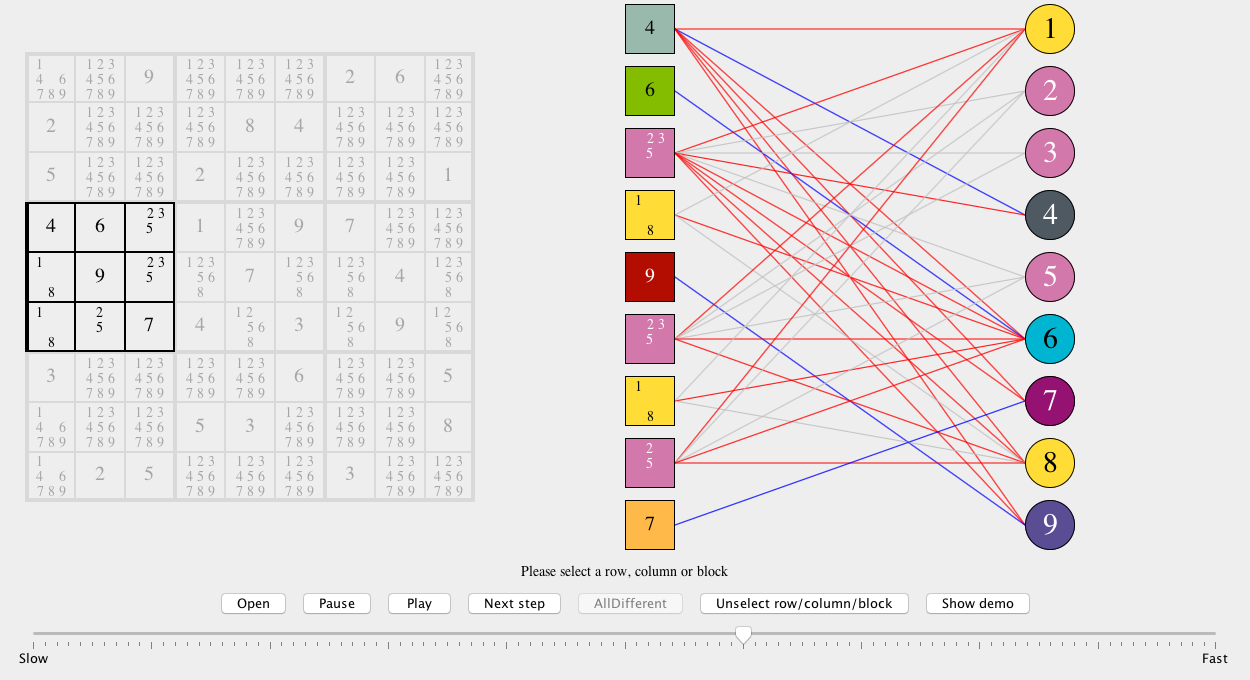
\includegraphics[width=8cm]{images/proof_of_concept/4.png}}
\vspace*{2cm}
\hfill
%\caption{Title for both}
%\end{figure}

%\begin{figure}[h]
\hfill
\subfigure[1st column after running the all-different algorithm]{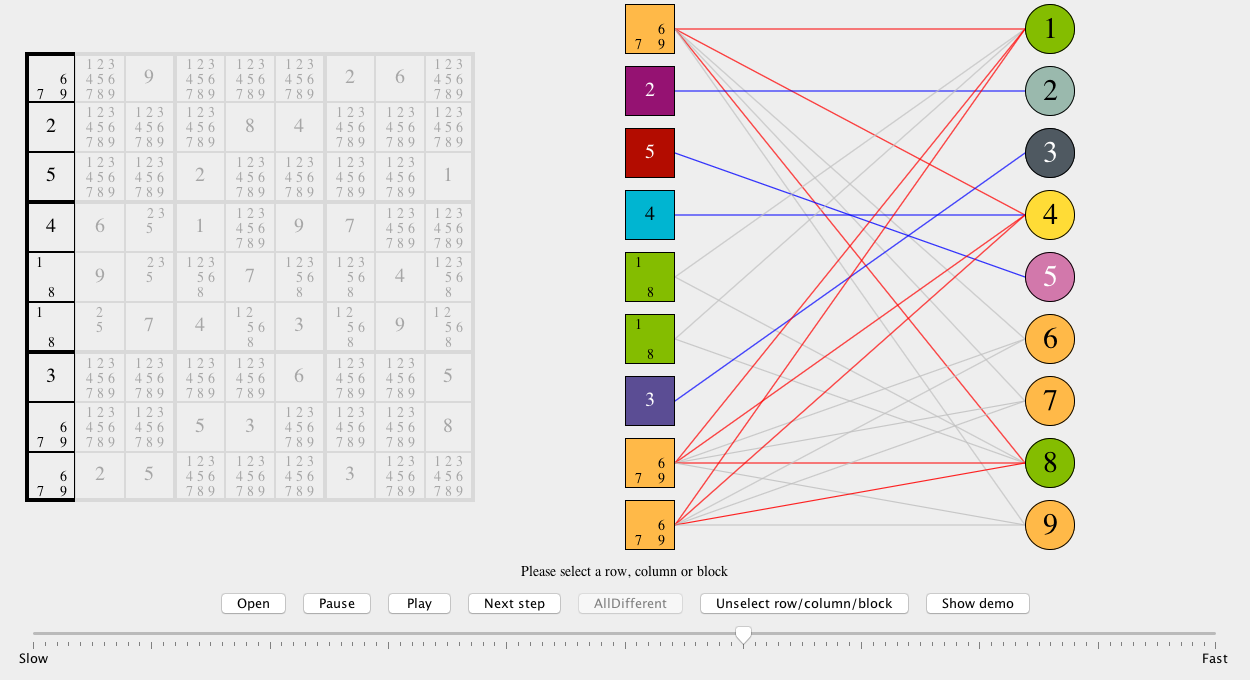
\includegraphics[width=8cm]{images/proof_of_concept/5.png}}
\hfill
%\subfigure[Proof]{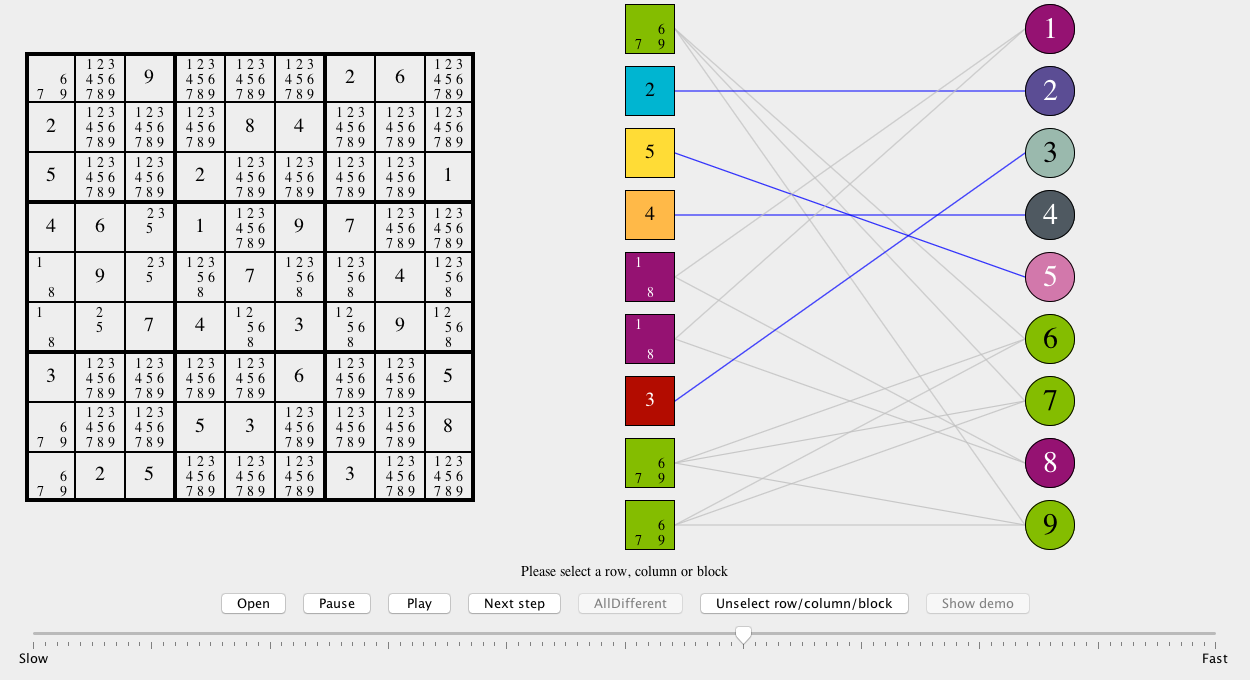
\includegraphics[width=8cm]{images/proof_of_concept/6.png}}
\hfill
\caption{Steps in the demo}
\label{fig:proof_1_5}
\end{figure}

\clearpage 

\begin{figure}[h]
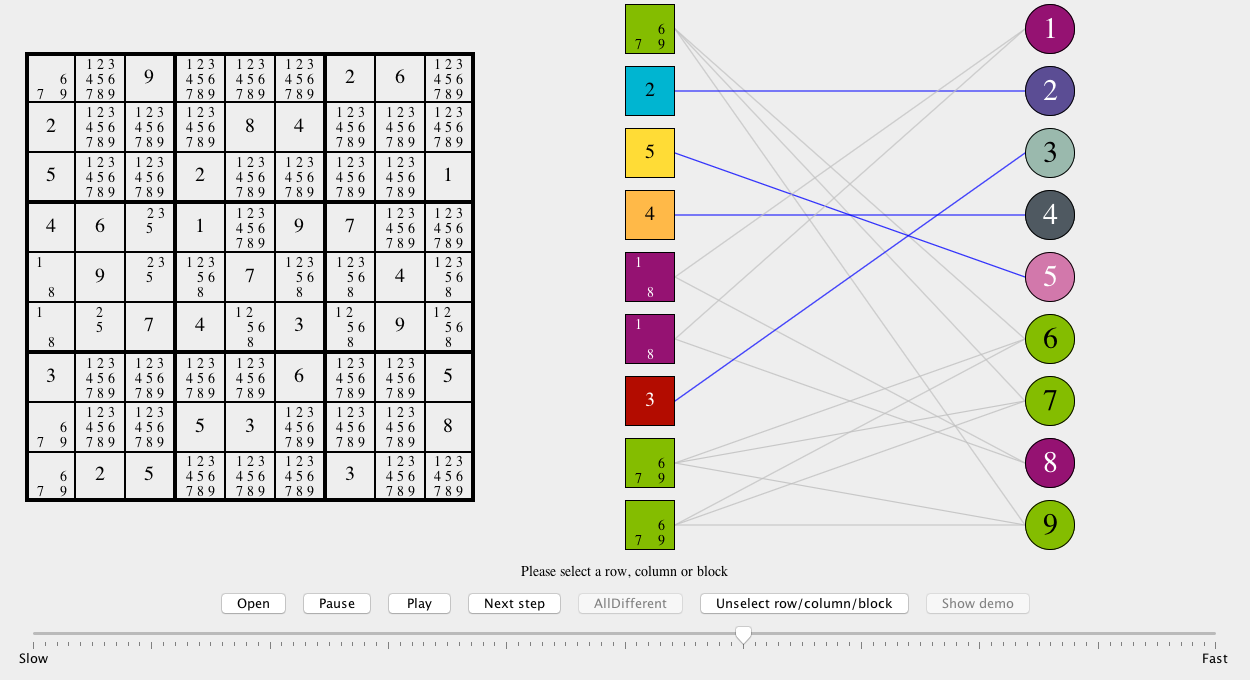
\includegraphics[width=16cm]{images/proof_of_concept/6.png}
\caption{State of the program after running the demo}
\label{fig:proof_6}
\end{figure}

As seen in ~\Cref{fig:proof_1_5}, the all-different algorithm performs changes only to the selected 9 cells  inside a row, column or 3x3 sub-grid. 

The end result of following the above steps can be seen in ~\Cref{fig:proof_6}. This state mimics the human thinking when solving a Sudoku. In the 1st column there are two cells with a domain of ${1, 8}$, but we don't know yet which cell will take which digit. What we do know though, is that the digits ${1, 8}$ will be distributed in that two particular cells, therefore in the last step, after running the all-different algorithm on the 1st column we can observe that the digits ${1, 8}$ disappear from the domains of the rest of the cells in the selection.

\end{appendices}

%%%%%%%%%%%%%%%%%%%%
%   BIBLIOGRAPHY   %
%%%%%%%%%%%%%%%%%%%%

\bibliographystyle{plain}
\bibliography{bib}

\end{document}
